\section{State of the Art}

possible citation \cite{kovzovic2023air}


\subsection{ADSB History}
In the early stages of civil aviation, air traffic controllers primarily relied on Primary Surveillance Radar (PSR) and Secondary Surveillance Radar (SSR) to monitor aircraft. However, with improvements in aircraft performance and the expansion of long-haul air routes, the limitations of PSR and SSR—such as restricted coverage, insufficient information accuracy, and delayed updates—gradually became apparent. These limitations not only increased the navigational difficulty for long-distance flights but also posed safety risks. For instance, in 1983, Korean Air Flight 007 deviated from its intended route due to insufficient radar coverage, navigation system malfunctions, and communication failures~\cite{icao_1993}, ultimately entering Soviet airspace and being shot down, resulting in a major aviation accident.

To address these challenges, the aviation industry gradually developed the Automatic Dependent Surveillance–Broadcast (ADS-B) system over several decades. ADS-B leverages the Global Navigation Satellite System (GNSS) and onboard sensors, integrating information such as barometric altitude, inertial navigation, and airspeed measurements to generate aircraft state parameters. These parameters, including identification codes, position, altitude, velocity, and flight intent, are periodically broadcast via onboard ADS-B equipment~\cite{olive2024filtering}. Compared with traditional radar, ADS-B offers higher accuracy, shorter update intervals, broader coverage, and lower infrastructure and maintenance costs. It significantly enhances situational awareness for both pilots and air traffic controllers while reducing the burden on ground surveillance infrastructure.

The development of ADS-B can be traced back to the 1970s. In 1992, the Radio Technical Commission for Aeronautics (RTCA) first proposed ADS-related technical specifications in DO-212~\cite{RCTA_DO-212}, identifying it as a candidate technology for future air traffic surveillance. The DO-242 standard~\cite{RCTA_DO-242} issued in 1998 further established the technical framework and performance requirements for ADS-B systems. Between 1996 and 2006, the Federal Aviation Administration (FAA) conducted the CAPSTONE project in Alaska~\cite{faa2000capstone}, demonstrating the potential of ADS-B to improve operational safety and efficiency in remote airspace. In 2003, the 11th Air Navigation Conference of the International Civil Aviation Organization (ICAO) formally recognized ADS-B as a critical surveillance technology for future air traffic management and promoted its standardization and adoption~\cite{icao_2003}.

Since 2010, ADS-B has gradually entered large-scale global deployment. Various countries have promoted its adoption through regulations. The FAA requires all aircraft operating in controlled airspace to be equipped with ADS-B Out~\cite{cfr91-225}; Europe has similarly mandated ADS-B under the SESAR framework~\cite{undertaking2009european}, expecting to increase European airspace capacity by 80–100\% by 2040. Australia~\cite{casa2010cao20-18} and Singapore have also implemented ADS-B mandates. In China, a national policy issued in 2015~\cite{caac2015adsb} required the installation of ADS-B equipment on commercial aircraft. Meanwhile, satellite-based ADS-B~\cite{melero2024satera} has enabled real-time and high-precision surveillance over approximately 70\% of global airspace, and open platforms such as the OpenSky Network~\cite{schafer2014bringing} provide large-scale ADS-B data resources for academic research.


\subsection{ADSB Data current usages}
review of the litterature.

what are the usages of ADSB data

What are the algorihtms, categories?
What are the cleaning process?


an overview of the current use of ADS-B data in the research domain, identifying and structuring clusters of algorithms in use;

 an analysis of the main trends in ADS-B data usage based on a systematic literature review;

 \subsubsection{Paper Selection}

This section describes the process of identifying, screening, and organizing research publications related to the application of ADS-B data. To ensure both representativeness and research quality, we focused on journals and conferences with high academic impact in the fields of air traffic management (ATM) and digital aviation. The primary sources include the \textit{Digital Avionics Systems Conference (DASC)}, \textit{SESAR Joint Undertaking Annual Conference}, \textit{Air Traffic Management Seminar (ATM Seminar)}, \textit{International Conference on Research in Air Transportation (ICRAT)}, \textit{Transportation Research Part C: Emerging Technologies}, \textit{IEEE Transactions on Intelligent Transportation Systems}, and the \textit{Journal of Air Transport Management (JATM)}. Literature retrieval was mainly conducted through academic databases such as IEEE Xplore, ScienceDirect, and Elsevier Scopus, as well as publicly available proceedings from the aforementioned conferences.

Considering that large-scale implementation and operational use of ADS-B systems began worldwide around 2012, this year was set as the starting point for the large-scale research phase of ADS-B data. Therefore, this study selected English-language publications issued between 2012 and December 2024 as the objects of analysis. We manually collected research that explicitly utilized real ADS-B flight data from the selected journals and conferences, excluding studies that relied solely on simulated or synthetic datasets.

The detailed screening process was as follows:

\begin{itemize}
    \item \textbf{Initial Screening:} Titles and abstracts were reviewed to confirm the study’s relevance to the aviation domain, such as airspace optimization, trajectory prediction, or conflict detection and avoidance (DAA).
    \item \textbf{Keyword Filtering:} Only papers containing the term ``ADS-B'' in the title, abstract, or keywords were retained.
    \item \textbf{Data Authenticity Criterion:} Studies were required to clearly indicate the use of real ADS-B datasets. Papers using only simulated or artificially generated trajectories were excluded.
    \item \textbf{Duplication and Accessibility Review:} Duplicate publications and inaccessible preprints were removed to ensure the reproducibility and verifiability of the results.
\end{itemize}

After multiple rounds of screening and manual verification, a total of 161 papers were collected, covering representative applications of ADS-B data across diverse research domains. The distribution of the selected studies by source is illustrated in Figure ~\ref{fig:placeholder}.

\begin{figure}
    \centering
    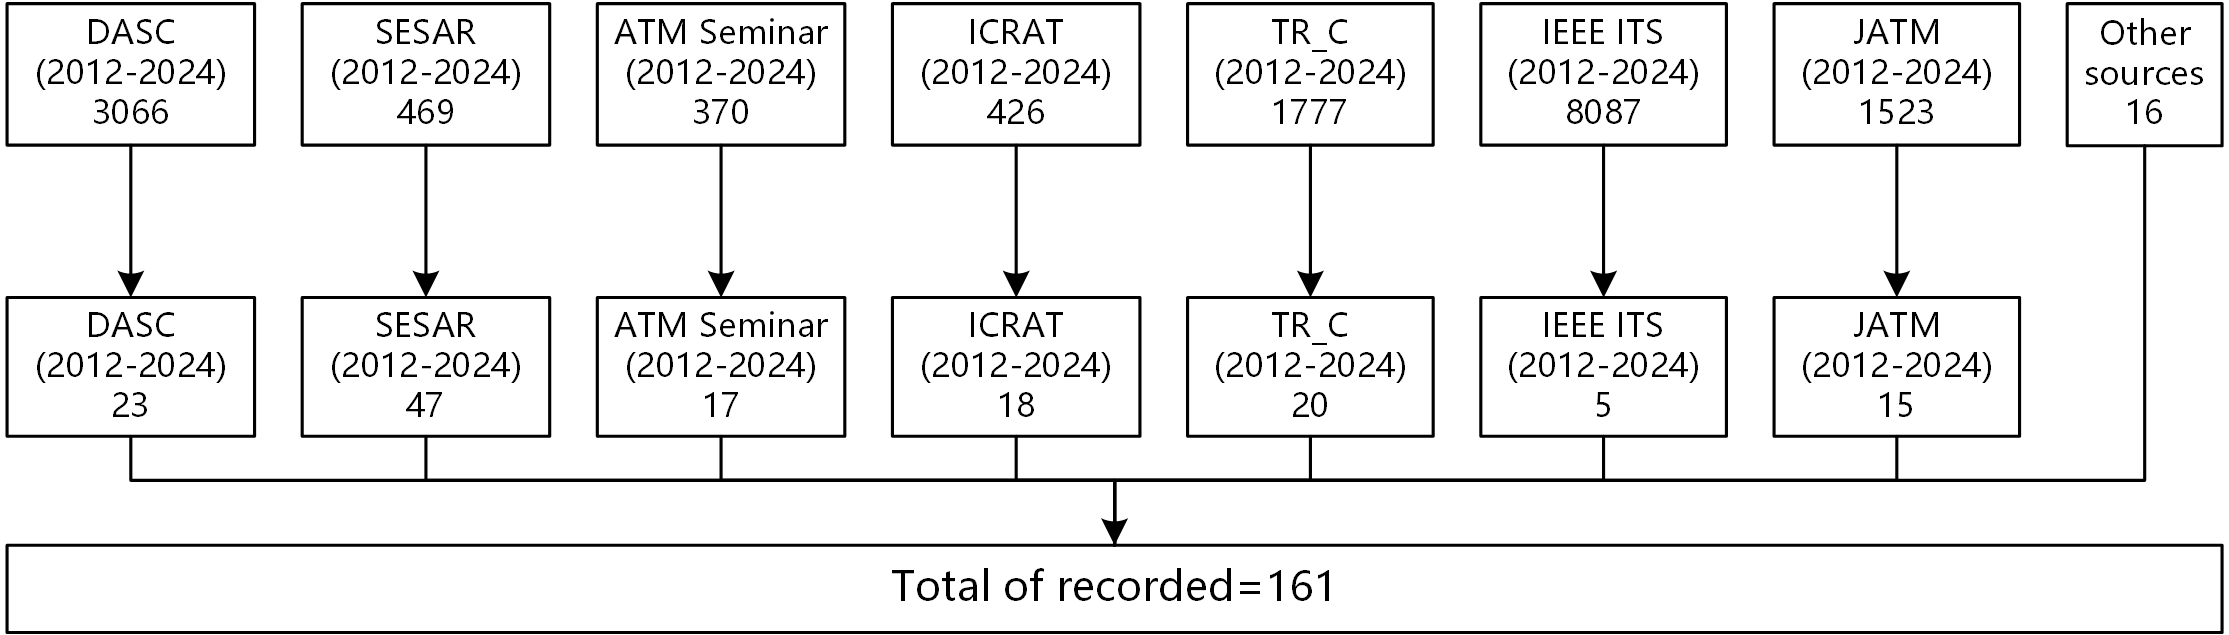
\includegraphics[width=1\linewidth]{paper_selection.png}
    \caption{Paper collection flow}
    \label{fig:placeholder}
\end{figure}
\subsubsection{Paper Clustering and Categorization}

The screened publications provided a solid data foundation for the categorization and trend analysis of ADS-B applications in this study. To systematically organize the characteristics and focal points of different research directions, we employed a mixed quantitative–qualitative approach for feature extraction and clustering of the collected literature.

Using Excel spreadsheets and reference management tools, the following key features were extracted from each selected conference and journal:
\begin{itemize}
    \item Publication year;
    \item Source conference or journal;
    \item Paper title and author keywords;
    \item Application scenario;
    \item Research focus or analytical perspective;
    \item Methods and algorithmic approaches (e.g., machine learning, optimization models, statistical analysis, simulation frameworks);
    \item Description of the ADS-B dataset used (e.g., public data repositories, airport-specific data, or crowdsourced datasets).
\end{itemize}

In the preliminary organization stage, the literature was grouped into four broad directions: trajectory prediction, air traffic management, aircraft performance estimation, and environmental sustainability. However, a subsequent systematic comparison and semantic analysis of all research features revealed significant overlaps and hierarchical relationships among different themes.

Therefore, this study adopted a combination of thematic synthesis and semantic grouping to reclassify the literature. This process comprehensively considered the research objectives, data utilization patterns, and the functional role of ADS-B within each study, aiming to establish a classification framework that systematically reflects the overall landscape of ADS-B research.

Finally, ADS-B–related studies were categorized into eight major domains:
Trajectory Modeling and Prediction, Operational Optimization and Management, Operational Safety and Surveillance, Aircraft Performance and Efficiency, Data Engineering and Enhancement, Environment and Sustainability, Security and Cybersecurity, Methodology, Simulation, and Policy

This classification framework provides the structural foundation for the domain-specific analysis presented in the following sections.


\textbf{Trajectory Modeling and Prediction.} 
This domain focuses on modeling historical and real-time aircraft trajectories and predicting their future states. The core tasks include 4D prediction, estimated time of arrival (ETA) calculation, trajectory pattern clustering and quantification of prediction uncertainty. As the core data source, ADS-B provides continuous, high-precision measurements of aircraft position, velocity, and altitude, forming the foundation for trajectory modeling and prediction. The data quality directly affects model accuracy and reliability. Gui et al. \cite{xuhao2021trajectory} proposed a semantic trajectory representation for arrival flight clustering to support airspace design, flow management, and ETA estimation; Wang et al. \cite{wang2017short} applied PCA-based dimensionality reduction and DBSCAN clustering for preprocessing, followed by a Multi-Cell Neural Network (MCNN) for short-term trajectory prediction in terminal maneuvering areas (TMA); and Wang et al. \cite{wang2018hybrid} integrated clustering-based preprocessing with hybrid MCNN models to improve ETA prediction accuracy.

\textbf{Operational Optimization and Management.} 
This domain focuses on improving the overall efficiency of airspace and airport operations, encompassing air traffic flow management, surface operations (taxiing and sequencing), terminal maneuvering area coordination, and airspace structure optimization. ADS-B data play a central role by providing continuous and fine-grained historical and real-time traffic information, serving as a reliable input for optimization models and decision-support systems. It enables accurate operational performance evaluation and data-driven strategy optimization. Research in this area often applies Mixed Integer Linear Programming, Simulated Annealing, and heuristic algorithms to address sequencing, scheduling, and routing problems. Other studies employ queuing models and Key Performance Indicators (KPIs) for operational assessment or mine historical ADS-B data to identify bottlenecks such as taxiway congestion and sector capacity limits. Basora et al. \cite{basora2018occupancy} developed a sector occupancy peak prediction model combining DBSCAN-based traffic flow clustering with Random Forest regression, and Delahaye et al. \cite{delahaye2022air} explored flow coordination at major intersections by applying hierarchical clustering to detect dominant flow patterns and using Transformer-based sequence modeling to support flow prediction and capacity management for air traffic controllers.

\textbf{Operational Safety and Surveillance.} 
This research domain focuses on ensuring aviation operational safety through enhanced situational awareness and data-driven analysis. Core topics include conflict detection and resolution (Detect and Avoid, DAA / ACAS), abnormal event detection (e.g., go-arounds, unstable approaches), operational risk assessment (such as collision risk and airspace complexity), and surveillance system performance evaluation. As an independent surveillance source, ADS-B data provide continuous and high-precision trajectory and state information, enabling real-time monitoring of aircraft behavior, detection of potential conflicts and anomalies, and quantitative assessment of operational safety. Bonifazi et al. \cite{bonifazi2021modeling} identified unstable approaches and go-arounds using ADS-B data, employing rule-based methods and Gaussian Mixture Models (GMM) for anomaly detection and integrating runway and weather information for improved accuracy. Rorie et al. \cite{rorie2024detect} conducted the first real-world evaluation of the ACAS Xr airborne collision avoidance system. Zhang et al. \cite{zhang2024study} investigated conflict-free routing strategies and compared multiple optimization algorithms, while Bao et al. \cite{bao2024exploring} proposed a multi-airport terminal area risk prediction framework to assess inter-airport conflict probabilities. Collectively, these works highlight the pivotal role of ADS-B data in safety assurance and operational surveillance research.

\textbf{Aircraft Performance and Efficiency.} 
This research area focuses on deriving aircraft performance parameters from flight data to calibrate or complement existing performance models such as BADA, and to assess energy efficiency across different aircraft types and operational phases. Key parameters include aircraft mass, drag polar, thrust settings, fuel consumption, and speed profiles. In this context, ADS-B data serve as a crucial source of flight state information—providing ground speed, vertical rate, and heading—that enables large-scale, fleet-level performance analysis even when detailed design parameters are unavailable. This facilitates more accurate and data-driven model validation and calibration. Sun et al. \cite{sun2018aircraft} proposed a stochastic hierarchical modeling framework combining Bayesian computation and Markov Chain Monte Carlo (MCMC) sampling to estimate drag polars from flight data, deriving zero-lift drag coefficients and induced drag factors. Schultz et al. \cite{schultz2022data} integrated FDR and ADS-B data to model aircraft fuel consumption and operational efficiency using CART and neural network models. Alligier et al. \cite{alligier2020predictive} predicted aircraft mass and speed intent during climb phases to improve physics-based ground trajectory prediction. Collectively, these studies demonstrate the essential role of ADS-B data in performance inversion, efficiency modeling, and validation of aircraft performance models.

\textbf{Data Engineering and Enhancement.} 
This category focuses on improving the quality and usability of raw ADS-B data, which serve as the foundation for subsequent analytical and modeling applications. Key tasks include data cleaning and anomaly detection, missing-value imputation, multi-source data fusion, data compression and indexing, and synthetic data generation. In this research domain, ADS-B data themselves are the core subject of engineering—aimed at producing cleaner, more complete, and more interoperable datasets that can support trajectory prediction, operational analysis, and safety evaluation. Tabassum et al. \cite{tabassum2017ads} performed long-term statistical analysis and anomaly identification on ADS-B messages and basic reports, revealing the effects of systematic errors and signal loss on trajectory accuracy. Wandelt et al. \cite{wandelt2018ads} proposed an efficient compression and indexing scheme for large-scale ADS-B records to enable real-time querying and scalable analytics. Spinielli et al. \cite{spinielli2017initial} led by the EUROCONTROL Performance Review Unit (PRU), developed an open and reproducible reference trajectory dataset for operational performance assessment, integrating multiple data sources including ADS-B, CPR, airport data, and Network Manager (NM) information. Collectively, these studies have advanced ADS-B data from raw collection toward structured, reliable research assets.

\textbf{Environment and Sustainability}
This research area focuses on quantifying the environmental impact of aviation operations and exploring sustainable optimization strategies, including greenhouse gas and pollutant emission assessment, contrail formation detection and avoidance, and noise evaluation. Owing to its wide coverage and high temporal resolution, ADS-B data serve as a crucial source for environmental modeling and validation. For instance, Roosenbrand et al. \cite{roosenbrand2023contrail} proposed a method to estimate contrail altitudes using shadows in Landsat satellite imagery, with ADS-B data employed as ground truth for validation. Sun et al. \cite{sun2023evaluating} integrated satellite-based and ground-based ADS-B data with wind field information to improve emission estimation and compared actual flight trajectories with optimal routes to quantify excess emissions.

\textbf{Security and Cybersecurity}
This domain focuses on identifying and mitigating cybersecurity threats targeting the ADS-B system itself, such as False Data Injection Attacks (FDIA), signal spoofing, and message tampering, to ensure the integrity and reliability of surveillance information. In this field, the ADS-B protocol, signal, and data link are the direct subjects of vulnerability analysis and protection technology research. For example, Cretin et al. \cite{cretin2018increasing} proposed a Domain-Specific Language (DSL)-based testing framework to evaluate the resilience of Air Traffic Control (ATC) systems against FDIA, while Khan et al. \cite{khan2021intrusion} employed machine learning techniques for ADS-B intrusion detection.

\textbf{Methodology, Simulation, and Policy}
This category provides foundational tools, frameworks, and policy support for aviation research. It includes the development of open-source simulation platforms, advocacy of reproducible research practices, establishment of data standards, and discussion of regulatory and privacy issues related to ADS-B deployment. In this context, ADS-B serves both as input data for constructing realistic scenarios in simulation environments and as a focal topic in advancing data-sharing policies, privacy protection, and industry standards. For example, Mehlitz et al. \cite{mehlitz2019analyzing} proposed the RACE framework for comprehensive airspace data analysis, while Bolic et al. \cite{bolic2024roadmap} systematically elaborated on the European ATM Open Science Alliance and its Open Performance Data Initiative (OPDI).

 
\begin{table*}[htbp]
\centering
\caption{Summary of ADS-B Application Categories, Main Methods, and Data Roles}
\begin{tabular}{p{3cm} p{6cm} p{3cm}}
\hline
\textbf{Category} & \textbf{Main Methods} & \textbf{Role of ADS-B Data} \\
\hline
\textbf{Trajectory Modeling and Prediction} &
\makecell[l]{Clustering (DBSCAN, K-means)\\
LSTM/Transformer prediction\\
Autoencoder feature extraction\\
DTW\\
PCA\\
Hybrid physical–data models} &
\textbf{Core data source} \\
\hline

\textbf{Operational Optimization and Management} &
\makecell[l]{
MILP\\
Simulated annealing\\
Heuristic algorithms\\
KPI-based performance metrics\\
Historical traffic analysis
} &
\textbf{Real-time/historical traffic input} \\
\hline

\textbf{Operational Safety and Surveillance} &
\makecell[l]{
DAA geometric models\\
Anomaly detection (thresholds, clustering, autoencoder, GMM)\\
Monte Carlo risk evaluation
} &
\textbf{Flight monitoring and safety baseline} \\
\hline

\textbf{Aircraft Performance and Efficiency} &
\makecell[l]{
Dynamic equation inversion\\
Maximum likelihood estimation\\
Bayesian inference\\
Particle filtering\\
Regression and neural networks
} &
\textbf{Model calibration data source} \\
\hline

\textbf{Data Engineering and Enhancement} &
\makecell[l]{
Kalman filtering\\
Map-matching\\
Multisource fusion\\
Data indexing\\
Generative models (TimeGAN)
} &
\textbf{Primary processing object} \\
\hline

\textbf{Environment and Sustainability} &
\makecell[l]{
Trajectory-based emission estimation\\
Remote sensing data fusion\\
Optimal control route planning
} &
\textbf{Environmental assessment input} \\

\textbf{Security and Cybersecurity} &
\makecell[l]{
Intrusion detection (ML classifiers)\\
Protocol vulnerability testing\\
SDR signal analysis
} &
\textbf{Research target} \\
\hline

\textbf{Methodology, Simulation, and Policy} &
\makecell[l]{
Open-source simulation platform development\\
Data standardization\\
Policy and privacy analysis
} &
\textbf{Research infrastructure and policy object} \\
\hline
\end{tabular}
\label{tab:adsb_applications}
\end{table*}


 %\subsection{ADSB Data future usages}